\section{Exclusion Heuristic Validation: RQ3}
\label{sec:pareto_and_weights}
\subsection{Baseline Gain and Component Ablations}
On the original graph, the direct heuristic yields $P=1{,}022$ at budget 100, compared with greedy coverage's 800 and exact union's 534. This gain comes with $C=5{,}020$ and $H=13.23\%$; it does not maximize every objective. Table~\ref{tab:q1_supermodular_p} retains the multi-budget comparison.
% Auto-generated Supermodular P(S) Optimization Table for Q1 Journal Expansion
\begin{table*}[t]
\centering
\small
\caption{All-source exclusion $P(S)$ optimization via greedy minimum-source heuristic versus baseline single-objective rankings.}
\label{tab:q1_supermodular_p}
\begin{tabular}{rrrrrrrr}
\toprule
Budget & \multicolumn{3}{c}{Direct $P(S)$ Heuristic} & Greedy $P$ & Union $P$ & Gain vs Gr. & Gain vs Un.\\
\cmidrule(lr){2-4}
$|S|$ & $P$ & $C$ (\%) & $H$ (\%) & & & $\Delta P$ & $\Delta P$\\
\midrule
10 & \textbf{479} & 55.4\% & 2.58\% & 351 & 343 & +128 & +136\\
25 & \textbf{618} & 59.1\% & 4.15\% & 514 & 427 & +104 & +191\\
50 & \textbf{803} & 64.2\% & 6.55\% & 638 & 441 & +165 & +362\\
100 & \textbf{1,022} & 70.0\% & 13.23\% & 800 & 534 & +222 & +488\\
\bottomrule
\end{tabular}
\end{table*}


\begin{figure}[t]
\centering
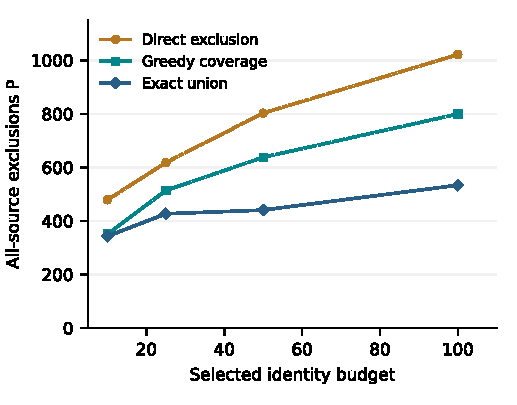
\includegraphics[width=\columnwidth]{q1_supermodular_p.pdf}
\caption{All-source exclusion under the original heuristic and coverage/exposure baselines. Counts describe the retained graph under ideal selected-source hardening.}
\label{fig:q1_supermodular_p_weights}
\end{figure}

The new runner parameterizes the original lexicographic rule and reproduces its complete retained 100-account order before introducing variants. It changes the candidate cap to 1, 5, 20 and unrestricted, removes reciprocal remaining-source scoring or the coverage tie-break, and repeats tied choices under 30 frozen seeds. These are component sensitivities, not independent ecosystem observations.
% Generated by scripts/render_journal_validation.py
\begin{table*}[t]
\centering
\footnotesize
\caption{Budget-100 component ablations on the original graph. Timing is one selection run in the same process.}
\label{tab:revision_heuristic}
\begin{tabular}{lrrrr}
\toprule
Rule & $C$ & $H$ (\%) & $P$ & Seconds\\
\midrule
Original rule (cap 10) & 5,020 & 13.23 & 1,022 & 19.56\\
Immediate + coverage & 5,043 & 11.75 & 1,024 & 13.65\\
No coverage tie-break & 5,020 & 13.23 & 1,022 & 13.64\\
Cap 1 & 5,020 & 13.23 & 1,022 & 4.96\\
Cap 5 & 5,020 & 13.23 & 1,022 & 11.45\\
Cap 20 & 5,020 & 13.23 & 1,022 & 17.63\\
No candidate cap & 5,020 & 13.23 & 1,022 & 89.10\\
\bottomrule
\end{tabular}
\par\smallskip\begin{minipage}{0.98\textwidth}\footnotesize Immediate + coverage omits reciprocal remaining-source scoring and is identical to the no-reciprocal variant. Thirty seeded tie runs each give $P=1{,}022$ at budget 100; this is selection variability on one graph, not ecosystem uncertainty.\end{minipage}
\end{table*}


Removing reciprocal scoring gives $P=1{,}024$, two more than the original rule, together with $C=5{,}043$ and $H=11.75\%$. The immediate-completion variant uses coverage then identity order to resolve zero-gain cases. Candidate-cap changes and removing the coverage tie-break retain the original budget-100 P on this graph. All 30 tie runs also yield $P=1{,}022$. These outcomes provide no evidence that the reciprocal term improves original-graph exclusion; its usefulness must be assessed across other observed populations. Single-run timing in Table~\ref{tab:revision_heuristic} characterizes the implementation rather than a hardware-independent performance guarantee.

\subsection{Candidate-Restricted Exact Benchmarks}
We freeze 20 empirical candidate pools and 12 synthetic overlap instances, each with 20 eligible accounts and budgets 1, 3 and 5. Exhaustive enumeration evaluates every eligible subset. Empirical instances preserve complete endpoint source sets: sources outside the candidate pool remain unselected and can prevent exclusion. Candidate pools are constructed from low-cardinality source sets and reach-ranked fill accounts, so these are tractable diagnostic instances rather than a random sample of full-graph optimization problems.
% Generated by scripts/render_journal_validation.py
\begin{table*}[t]
\centering
\footnotesize
\caption{Exact exclusion benchmarks with 20 eligible accounts and budgets 1, 3 and 5.}
\label{tab:revision_exact}
\begin{tabular}{lrrrr}
\toprule
Instance family & Settings & Exact hits & Worst gap & Min ratio (\%)\\
\midrule
Empirical candidate pools & 60 & 51 & 66 & 16.46\\
Synthetic overlap instances & 36 & 35 & 1 & 93.33\\
\bottomrule
\end{tabular}
\par\smallskip\begin{minipage}{0.98\textwidth}\footnotesize Twenty empirical pools and twelve synthetic instances each supply three correlated budget settings. Outside-candidate sources remain unselected. Optima apply only to the restricted instance; no full-graph approximation guarantee follows.\end{minipage}
\end{table*}


The original heuristic reaches the restricted optimum in \HeuristicExactHits{} of \HeuristicExactSettings{} settings. It matches 51 of 60 empirical settings and 35 of 36 synthetic settings. Its worst empirical deficit is \HeuristicWorstGap{} endpoints and its minimum achieved-to-optimal ratio is 16.46\%; the worst synthetic deficit is one endpoint. Figure~\ref{fig:revision_audit_benchmarks}(b) shows the gap distributions. The 96 settings reuse 32 instances across budgets and are not independent replicates. These diagnostics identify substantive failure cases; neither the hit count nor the synthetic results certify the original full graph's optimum or an approximation ratio.

\subsection{Other Objective Choices}
Standard scalarization exposes intermediate coverage--exposure choices, but a preferred weight requires review costs and stakeholder preferences that were not measured. Additional heterogeneous weights, strict thresholds and uniform-efficacy multipliers are reported in Appendix~\ref{sec:objective_supplement}. A threshold sensitivity is not a count of empirically protected repositories: source identities are not authenticated approval groups, and the study does not observe an enforced release policy.
